\documentclass{article}
\usepackage{amsmath}
\usepackage{graphicx}
\usepackage{tikz}
\usepackage{pgfplots}
\pgfplotsset{compat=1.18}

\title{Graphing Equations}\\
\author{Tutoring Centre Ferndale\\

\includegraphics[width=4em]{ApS_logo.png}}
\date{}\\

\begin{document}

\maketitle

\section*{Dimensions}
Dimensions are measurements of the size of things.
\begin{itemize}
    \item To measure just the length of something you need only one dimension.
    \item To measure something flat you will need to measure the two dimensions of length and width. That's why flat things are said to be 2D or two-dimensional.
    \item To measure the size of solid objects that have some volume you will need to measure the three dimensions of length, width, and height. That's why they are said to be 3D or three-dimensional.
\end{itemize}
You can think of dimensions as the number of independent directions in which movement or measurement can occur within a space.

\section*{Axes}
An axis is an imaginary line around which something else revolves, such as the axis of the Earth or the axis of the stars. Navigators and astronomers use these lines as a reference in recording the locations of things.

\begin{itemize}
    \item Axis is a Latin word so the plural of "axis" is "axes," pronounced "ax-ees."
\end{itemize}

Mathematicians extended the idea of axes to mean any line used to define the positions of points in space. Each axis represents a dimension of the space and provides a scale for measuring distances and directions relative to it. The number of axes required corresponds to the number of dimensions in the space.

\newpage

\section*{Types of Spaces}

\paragraph{Lines}
A line has only one dimension. There is only one possible direction for movement along the line. There is length but no width or height.

\bigskip

\begin{center}
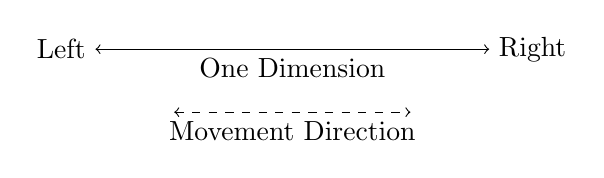
\begin{tikzpicture}
    \draw[<->] (0,0) -- (5,0);
    \node[left] at (0,0) {Left};
    \node[right] at (5,0) {Right};
    \node[below] at (2.5,0) {One Dimension};
    \draw[<->, dashed] (1,-0.8) -- (4,-0.8);
    \node[below] at (2.5,-0.8) {Movement Direction};
\end{tikzpicture}
\end{center}

\bigskip

\paragraph{Planes}
A plane has two dimensions. There are two possible directions of motion on a flat plane: There is length and width in this space, but no height. You can go forwards and backwards, or you can go left and right. There is no up or down.

\bigskip

\begin{center}
\begin{tikzpicture}
    \node[left] at (-1,0) {Left};
    \draw[<->] (-1,0) -- (5,0);
    \node [right] at (5,0) {Right};
    
    \node[above] at (0,5) {Up};
    \draw[<->] (0,-1) -- (0,5);
    \node[below] at (0,-1) {Down};
    
    \node[below] at (2.5,0) {Dimension};
    \node[left, rotate=90] at (-.3,3) {Dimension};
    \draw[<->, dashed] (1.5,1) -- (4,1);
    \draw[<->, dashed] (1,1.5) -- (1,4);
    \node[below] at (2.7,1) {Movement Direction};
    \node[left, rotate=90] at (0.7,4.5) {Movement Direction};
\end{tikzpicture}
\end{center}

\newpage

\paragraph{Cubes}
A cube has three dimensions. There are three possible directions of motion within the space of a cube: You can go forwards and backwards, or you can go left and right, or you can go up and down.

\bigskip

\begin{center}
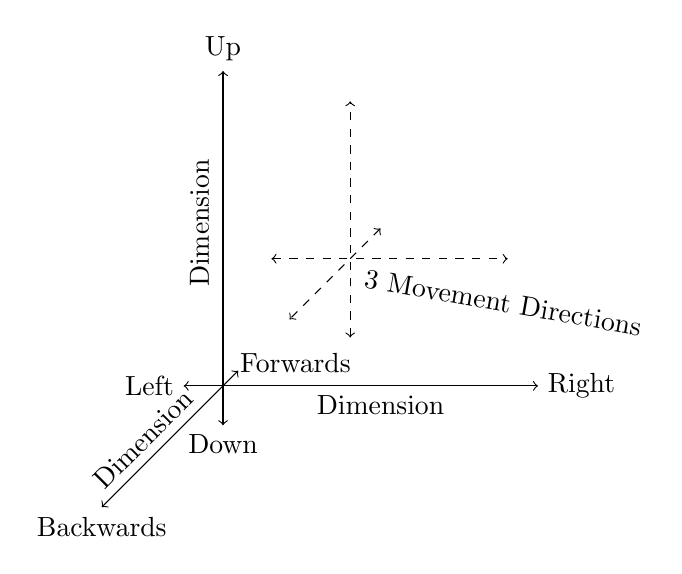
\begin{tikzpicture}
    \node[left] at (-.5,0,0) {Left};
    \draw[<->] (-.5,0,0) -- (4,0,0);
    \node[right] at (4,0,0) {Right};
    \node[above] at (0,4,0) {Up};
    \draw[<->] (0,-.5,0) -- (0,4,0);
    \node[below] at (0,-.5,0) {Down};
    \node[right] at (-.1,0.1,-.5) {Forwards};
    \draw[<->] (0,0,-.5) -- (0,0,4);
    \node[below] at (0,0,4) {Backwards};
    \node[below] at (2,0,0) {Dimension};
    \node[left, rotate=90] at (-0.3,3,0) {Dimension};
    \node[above , rotate=45] at (0,0,2.2) {Dimension};
    \draw[<->, dashed] (1,2,1) -- (4,2,1);
    \draw[<->, dashed] (2,1,1) -- (2,4,1);
    \draw[<->, dashed] (2,2,0) -- (2,2,3);
    \node[below, rotate=-10] at (3.6,1.3,0) {3 Movement Directions};
\end{tikzpicture}
\end{center}

\section*{Cartesian Coordinates}

\begin{itemize}
    \item To coordinate means to work with someone or something else. Coordinates in maths are sets of numbers that work together to mark an exact location on the space defined by axes.
    \item Sets of numbers used this way are called Cartesian coordinates. They are named after the French mathematician and philosopher Renee Descartes who wrote about them in an important book in 1637. His book popularized the idea of coordinates and made it possible to use algebra to solve problems of geometry.
    \item Dimensions are the number of independent directions in which we can move or measure, and they determine the number of coordinates needed to specify a point's position within that space.
\end{itemize}

\newpage

\subsection*{Spaces and Dimensions\\using Cartesian Coordinates}

\begin{enumerate}
    \item One-Dimensional (1D) Space:

   - Involves a single axis, usually represented as a line.
   
   - A point in this space is described by one number, usually named \( x \).

\item Two-Dimensional (2D) Space:

   - Involves two perpendicular axes: the \( x \)-axis (horizontal) and the \( y \)-axis (vertical).
   
   - A point in this space is described by a pair of coordinates, \( (x, y) \).
   
   - This forms a plane where any position can be defined by how far it is along the \( x \)-axis and \( y \)-axis.

\item Three-Dimensional (3D) Space:

   - Involves three perpendicular axes: the \( x \)-axis, \( y \)-axis, and \( z \)-axis.
   
   - A point in this space is described by a triple of coordinates, \( (x, y, z) \).
   
   - This forms a volume where any position can be defined by how far it is along the \( x \)-axis, \( y \)-axis, and \( z \)-axis.
\end{enumerate}

\section*{Dependent and Independent Variables}

\subsection*{Independent Variable}

The independent variable is the variable that you, as the experimenter or observer, can control or manipulate. It is plotted along the horizontal axis (the x-axis) of a graph. In the equation \( y = mx + b \), the independent variable is \( x \).

\begin{itemize}
    \item The independent variable is what you change or control.
    \item It is usually the input or cause in an experiment or relationship.
\end{itemize}

\subsection*{Dependent Variable}

The dependent variable is the variable that depends on the value of the independent variable. It is plotted along the vertical axis (the y-axis) of a graph. In the equation \( y = mx + b \), the dependent variable is \( y \).

\begin{itemize}
    \item The dependent variable is what you measure or observe.
    \item It is usually the output or effect in an experiment or relationship.
\end{itemize}

When graphing equations, understanding which variable is independent and which is dependent helps in correctly setting up and interpreting the graph.

\section*{Graphing Equations}

To graph an equation, we plot points that satisfy the equation on the Cartesian plane. 

Consider the equation \( y = 2x + 1 \):

\begin{itemize}
    \item Here, \( x \) is the independent variable. You choose different values for \( x \) to see how \( y \) changes.
    \item \( y \) is the dependent variable. Its value depends on the chosen values of \( x \).
\end{itemize}

We can create a table of values for $x$ and corresponding values for $y$:

\vspace{12pt}

\begin{center}
\resizebox{0.4\textwidth}{!}{
\begin{tabular}{|c|c|c|c|c|c|}
\hline
$x$ & -2 & -1 & 0 & 1 & 2 \\
\hline
$y$ & -3 & -1 & 1 & 3 & 5 \\
\hline
\end{tabular}
}
\par\vspace{1em}
\large{$y=2x+1$}
\end{center}

This table gives a set of Cartesian Coordinates that can be plotted onto a pair of axes. Drawing a line through the plotted points then gives all possible solutions for the equation.

\begin{center}
\begin{tikzpicture}[domain/.style={domain, very thick, smooth}]
    \draw[thick,<->] (-5,0) -- (5,0) node[right] {$x$ (independant variable)};
    \draw[thick,<->] (0,-3.5) -- (0,5) node[above] {$y$ (dependant variable)};
    \foreach \x in {1,...,4}
	\draw (\x,4pt) -- +(0,-8pt) node [below] {$\x$};
    \foreach \x in {-4,...,-1}
	\draw (\x,4pt) -- +(0,-8pt) node [below] {$\x$};
    \foreach \y in {1,...,4}
	\draw (4pt,\y) -- +(-8pt,0) node [left] {$\y$};
    \foreach \y in {-3,...,-1}
	\draw (4pt,\y) -- +(-8pt,0) node [left] {$\y$};
        \draw[domain, thick, <->] (-2,-3) -- (2,5) 
    node[pos=0.85, sloped, below] {$y=2x+1$};
    \foreach \x in {-4,...,4} \draw[width=.3pt, draw=gray!50] (\x,-3) -- (\x,5);
    \foreach \y in {-3,...,4} \draw[width=.3pt, draw=gray!50] (-5,\y) -- (5,\y);
\end{tikzpicture}
\end{center}

\newpage

\subsubsection*{Practical Example: Distance Over Time}

Suppose you are walking at a constant speed. The distance you travel over time can be modeled by the linear equation \( y = mx + b \), where:
\begin{itemize}
    \item \( x \) (independent variable) represents time in hours.
    \item \( y \) (dependent variable) represents distance in kilometres.
    \item \( m \) represents the speed of the car (kilometres per hour).
    \item \( b \) represents the starting distance (initial position) when \( x = 0 \).
\end{itemize}

\begin{center}
\begin{tikzpicture}[domain/.style={domain, very thick, smooth}]
    \draw[thick,<->] (-5,0) -- (5,0) node[right] {$x$ (hours of travel)};
    \draw[thick,<->] (0,-5) -- (0,5) node[above] {$y$ (kilometres travelled)};
    \foreach \x in {1,...,4}
	\draw (\x,4pt) -- +(0,-8pt) node [below] {$\x$};
    \foreach \x in {-4,...,-1}
	\draw (\x,4pt) -- +(0,-8pt) node [below] {$\x$};
    \foreach \y in {1,...,4}
	\draw (4pt,\y) -- +(-8pt,0) node [left] {$\y$};
    \foreach \y in {-4,...,-1}
	\draw (4pt,\y) -- +(-8pt,0) node [left] {$\y$};
        \draw[domain, thick, <->] (-2,-3) -- (2,5) 
    node[pos=0.85, sloped, below] {$y=2x+1$};
    \foreach \x in {-4,...,4} \draw[width=.3pt, draw=gray!50] (\x,-5) -- (\x,5);
    \foreach \y in {-4,...,4} \draw[width=.3pt, draw=gray!50] (-5,\y) -- (5,\y);
\end{tikzpicture}
\end{center}

By understanding which variables are independent and dependent, you can accurately plot and interpret the relationship between time and distance. The exact distance travelled after any given length of time can be read directly from this graph. For example, after 1 hour, you would have walked 3 kilometres.

\newpage

\subsection*{Practice Questions}

\begin{enumerate}
    \item Identify the independent and dependent variables in the equation \( y = 3x + 2 \).
    \item For a science experiment measuring the growth of a plant over time, what are the independent and dependent variables?
    \item Given the equation \( y = 5x - 4 \), describe how you would plot the graph and label the axes.
\end{enumerate}

\subsection*{Answers}

\begin{enumerate}
    \item In the equation \( y = 3x + 2 \), \( x \) is the independent variable, and \( y \) is the dependent variable.
    \item In the plant growth experiment, time (days, weeks, etc.) is the independent variable, and the height of the plant is the dependent variable.
    \item For the equation \( y = 5x - 4 \):
    \begin{itemize}
        \item Choose values for \( x \) (independent variable) and calculate corresponding \( y \) values (dependent variable).
        \item Plot the points \((x, y)\) on the graph.
        \item Label the x-axis as the independent variable and the y-axis as the dependent variable.
    \end{itemize}
\end{enumerate}

\end{document}
